% Created 2012-07-30 一 15:17
\documentclass[11pt]{article}
\usepackage[utf8]{inputenc}
\usepackage[T1]{fontenc}
\usepackage{fixltx2e}
\usepackage{graphicx}
\usepackage{longtable}
\usepackage{float}
\usepackage{wrapfig}
\usepackage{soul}
\usepackage{textcomp}
\usepackage{marvosym}
\usepackage{wasysym}
\usepackage{latexsym}
\usepackage{amssymb}
\usepackage{hyperref}
\tolerance=1000
\providecommand{\alert}[1]{\textbf{#1}}

\title{GIT分支管理是一门艺术}
\author{HDC}
\date{\today}
\hypersetup{
  pdfkeywords={},
  pdfsubject={},
  pdfcreator={Emacs Org-mode version 7.8.11}}

\begin{document}

\maketitle

\setcounter{tocdepth}{3}
\tableofcontents
\vspace*{1cm}


\section{GIT,在技术层面上,绝对是一个无中心的分布式版本控制系统,但在管理层面上,我建议你保持一个中心版本库。}
\label{sec-1}

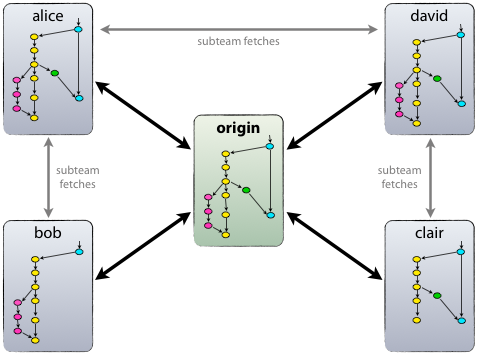
\includegraphics[width=.9\linewidth]{images/105017.png}
\section{我建议,一个中心版本库(我们叫它origin)至少包括两个分支,即“主分支”(master)和“开发分支”(develop)}
\label{sec-2}

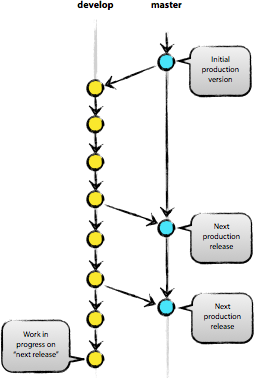
\includegraphics[width=.9\linewidth]{images/105026.png}
\section{要确保:团队成员从主分支(master)获得的都是处于发布状态的代码,而从开发分支(develop)应该总能够获得最新开发进展的代码}
\label{sec-3}
\section{在一个团队开发协作中,我建议,要有“辅助分支”的概念。}
\label{sec-4}
\section{“辅助分支”,大体包括如下几类:“管理功能开发”的分支、“帮助构建可发布代码”的分支、“可以便捷的修复发布版本关键BUG”的分支,等等}
\label{sec-5}
\section{“辅助分支”的最大特点就是“生命周期十分有限”,完成使命后即可被清除。}
\label{sec-6}
\section{我建议至少还应设置三类“辅助分支”,我们称之为“Feature branches”,“Release branches”,“Hotfix branches”。}
\label{sec-7}
\section{至此,我们形成了如下这张最重要的组织组,包含了两个粗体字分支(master/develop)和三个细体字分支(feature/release/hotfixes)。}
\label{sec-8}

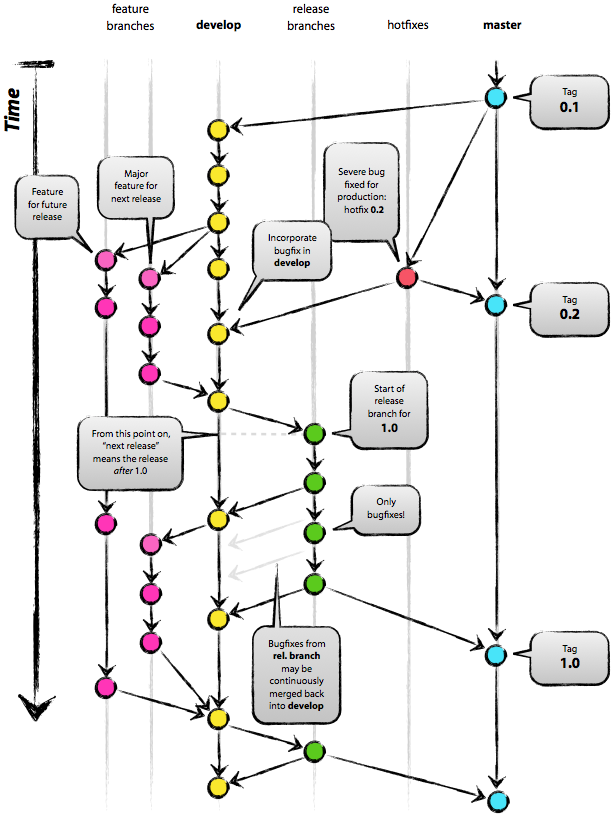
\includegraphics[width=.9\linewidth]{images/105037.png}
\section{“Feature branches”,起源于develop分支,最终也会归于develop分支。}
\label{sec-9}
\section{“Feature branches”常用于开发一个独立的新功能,且其最终的结局必须只有两个,其一是合并入“develop”分支,其二是被抛弃。最典型的“Feature branches”一定是存在于团队开发者那里,而不应该是“中心版本库”中。}
\label{sec-10}
\section{“Feature branches”起源于“develop”分支,实现方法是:}
\label{sec-11}


\begin{verbatim}
$ git checkout -b myfeature develop
\end{verbatim}
\section{“Feature branches”最终也归于“develop”分支,实现方式是:}
\label{sec-12}


\begin{verbatim}
$ git checkout develop
$ git merge --no-ff myfeature
(--no-ff,即not fast forward,其作用是:要求git merge即使在fast forward条件下也要产生一个新的 merge commit)
(此处,要求采用 --no-ff 的方式进行分支合并,其目的在于,希望保持原有“Feature branches”整个提交链的完整性)
$ git branch -d myfeature
$ git push origin develop
\end{verbatim}
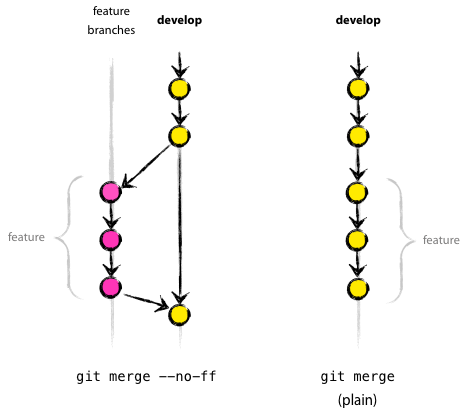
\includegraphics[width=.9\linewidth]{images/105048.png}
\section{“Release branch”,起源于 develo 分支,最终归于 “develop” 或 “master” 分支。这类分支建议命名为 “release-*”}
\label{sec-13}
\section{“Release branch” 通常负责 “短期的发布前准备工作”、“小bug的修复工作”、“版本号等元信息的准备工作”。与此同时,“develop”分支又可以承接一下个新功能的的开发工作了。}
\label{sec-14}
\section{“Release branch” 产生新提交的最好时候是 “develop” 分支已经基本到达预期的状态,至少希望新功能已经完全从 “Feature branches” 合并到 “develop” 分支了。}
\label{sec-15}
\section{创建 “Relase branches”,方法是:}
\label{sec-16}


\begin{verbatim}
$ git checkout -b release-1.2 develop
$ ./bump-version.sh 1.2 (这个脚本用于将代码所有涉及版本信息的地方都统一修改到 1.2,另外,需要用户根据自己的项目去编写适合的 bump-version.sh)
$ git commit -a -m "Bumped version number to 1.2"
\end{verbatim}
\section{在一段短时间内,在 “Release branches” 上,我们可以继续修复bug。在此阶段,严禁新功能的并入,新功能应该是被合并到 “develop” 分支的。}
\label{sec-17}
\section{经过若干 bug 修复后,“Release branches”上的代码已经达到可发布状态,此时,需要完成三个动作:第一是将 “Release branches” 合并到 “master” 分支,第二是一定要为 master 上的这个新提交打 TAG (记录里程碑),第三是要将 “Release branches” 合并回 “develop” 分支。}
\label{sec-18}


\begin{verbatim}
$ git checkout master
$ git merge --no-ff release-1.2
$ git tag -a 1.2 (使用 -u/-s/-a 参数会创建 tag 对象,而非软 tag)
$ git checkout develop
$ git merge --no-ff release-1.2
$ git branch -d release-1.2
\end{verbatim}
\section{“Hotfix branches” 源于 “master”,归于 “develop” 或 “master”,通常命令为 “hotfox-”}
\label{sec-19}
\section{“Hotfix branches” 类似于 “Release branch”,但产生此分支总是非预期的关键GUG。}
\label{sec-20}
\section{建议设立 “Hotfix branches” 的原因是:希望避免 “develop分支” 新功能的开发必须为BUG修复让路的情况。}
\label{sec-21}

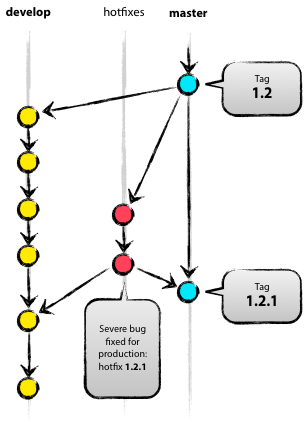
\includegraphics[width=.9\linewidth]{images/105059.png}
\section{建立 “Hotfix branches”,方法是:}
\label{sec-22}


\begin{verbatim}
$ git checkout -b hotfix-1.2.1 master
$ ./bump-version.sh 1.2.1
$ git commit -a -m "Bumpt version to 1.2.1" (然后可以开始问题修复工作)
$ git commit -m "Fixed severe production problem" (在问题修复后,进行第二次提交)
\end{verbatim}
\section{BUG修复后,需要将 “Hotfix branches” 合并回 “master” 分支,同时也需要合并回 “develop” 分支,方法是:}
\label{sec-23}


\begin{verbatim}
$ git checkout master
$ git merge --no-ff hotfix-1.2.1
$ git tag -a 1.2.1
$ git checkout develop
$ git merge --no-ff hotfix-1.2.1
$ git branch -d hotfix-1.2.1
\end{verbatim}

\end{document}
